\section{Feature 132}
\begin{figure}[h]
    \centering
    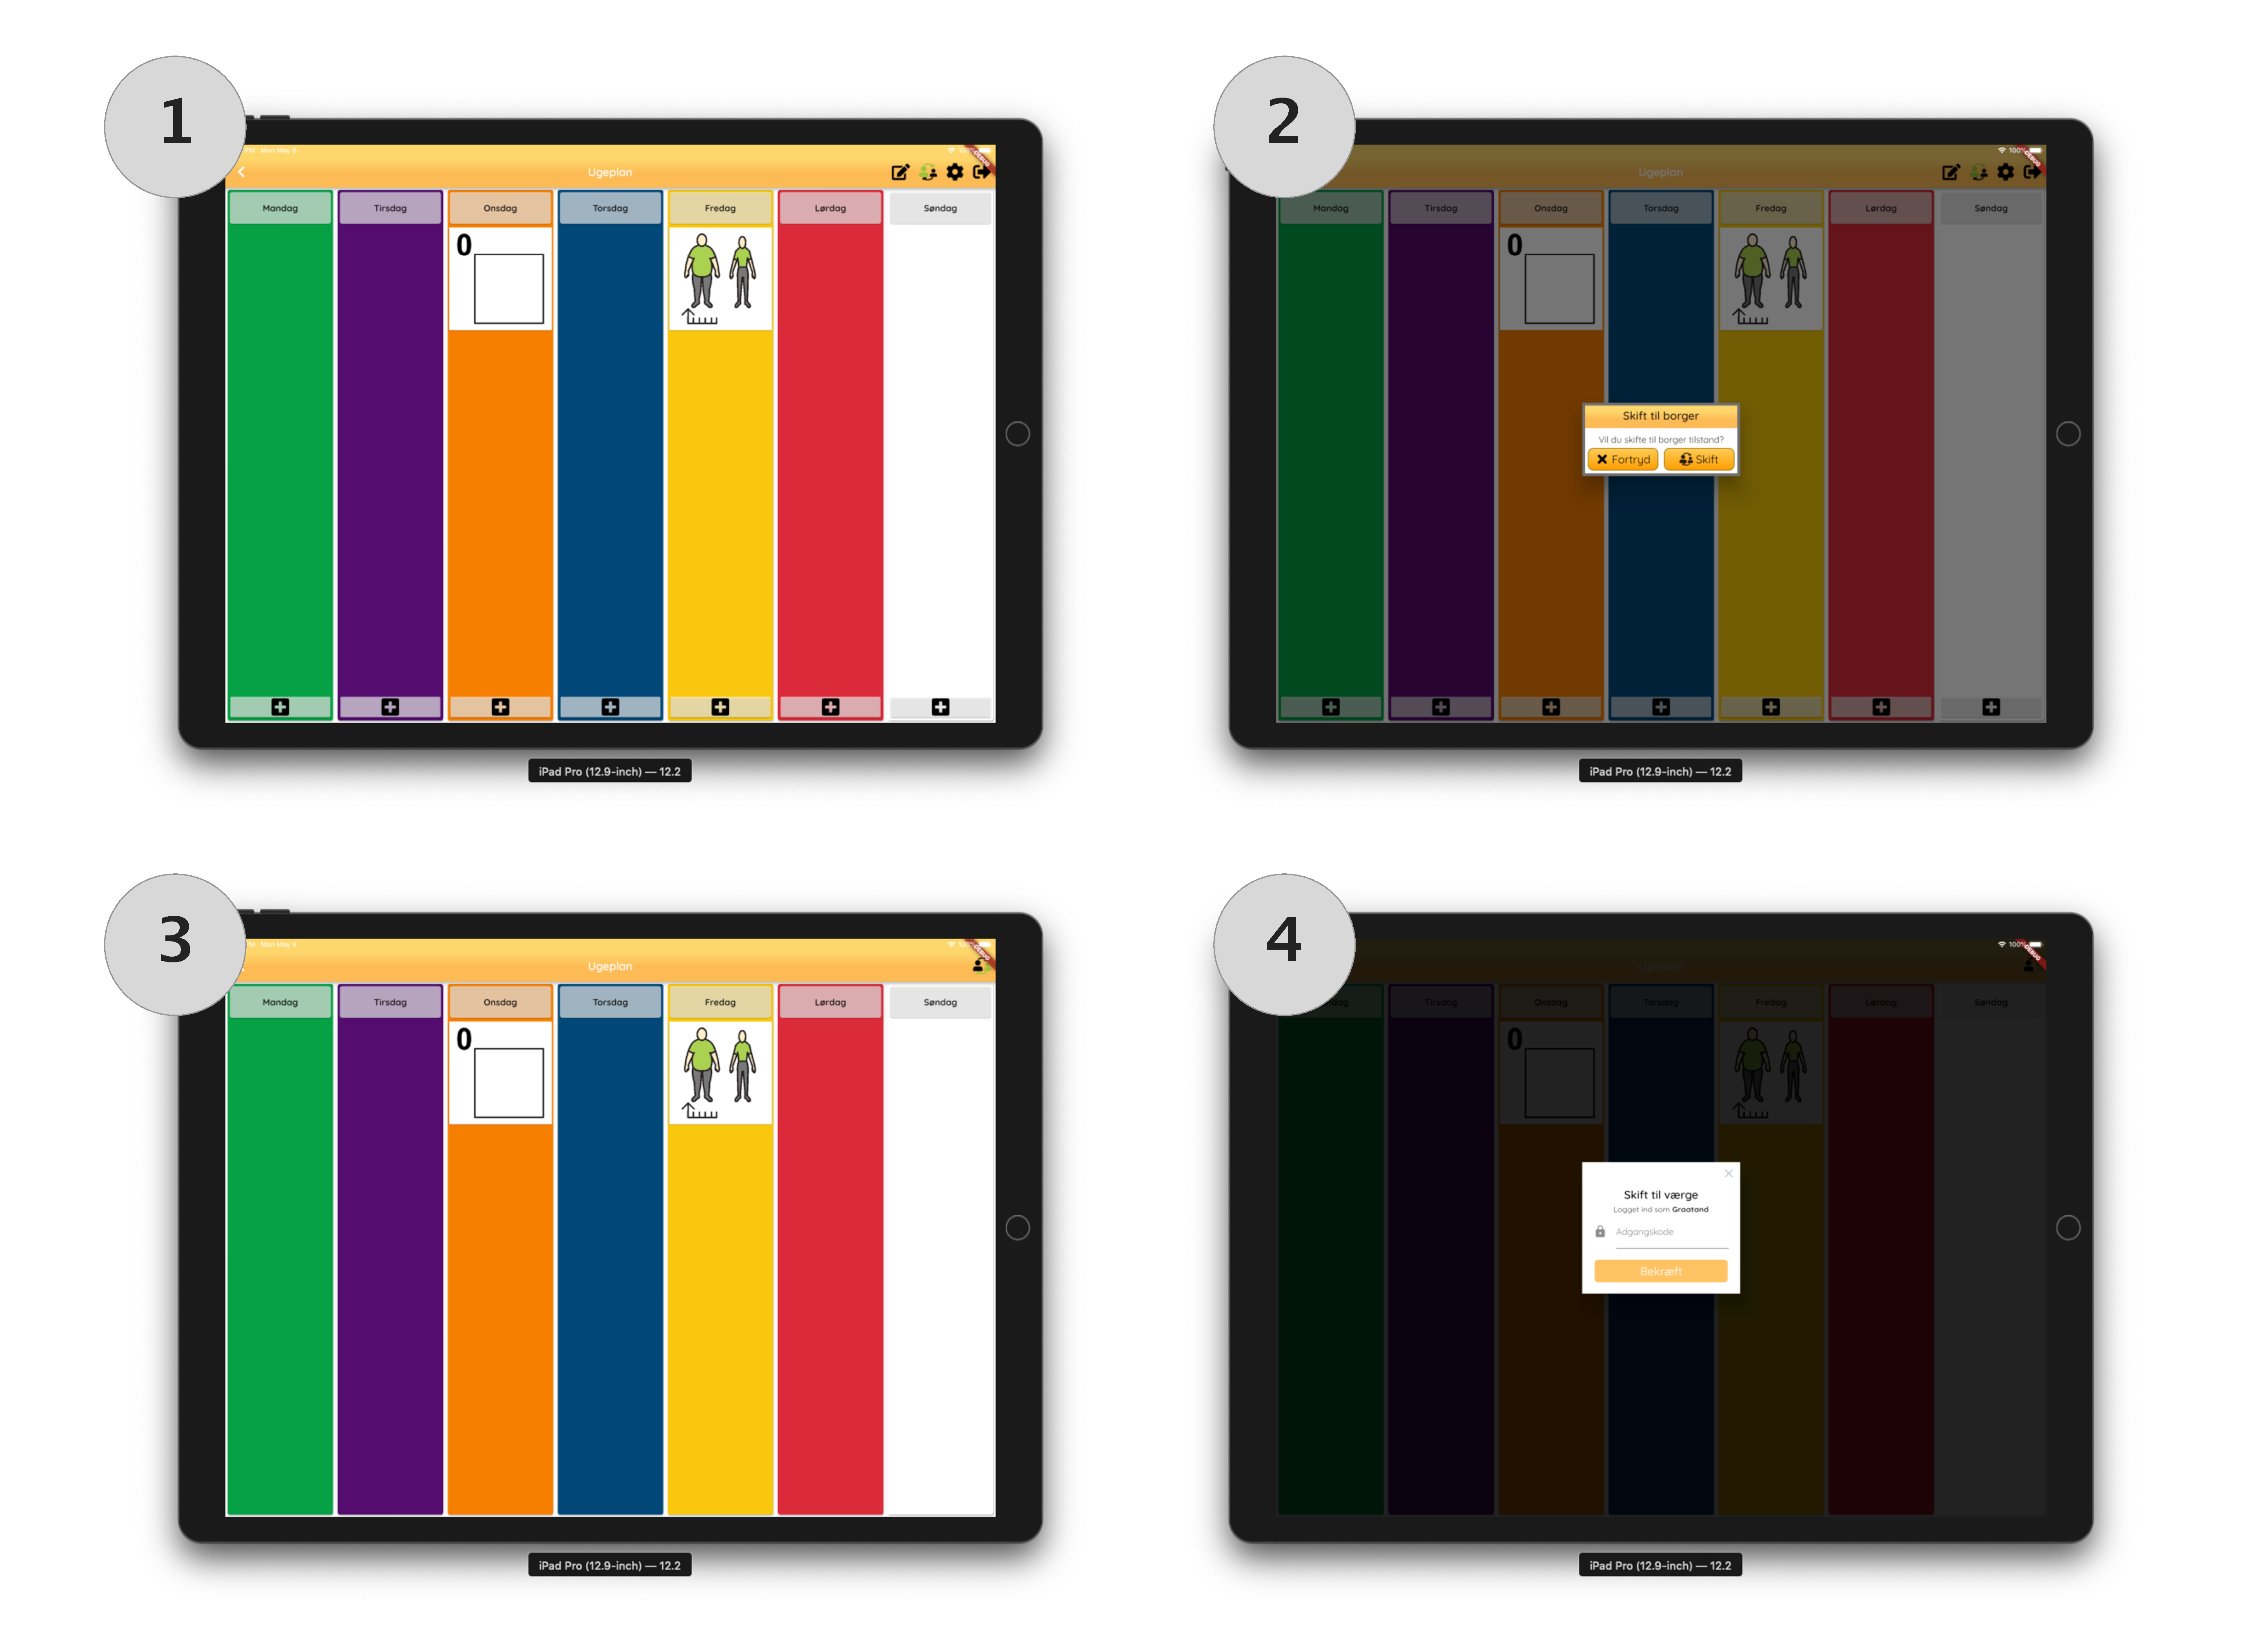
\includegraphics[width=0.8\textwidth]{figures/feature_132.pdf}
    \caption{An illustration of the final result after implementing feature 132}
    \label{fig:feature132}
\end{figure}

The feature was described as "As a user, I would like to be able to switch between guardian and citizen mode so that I can only access the parts of the system that I should be able to". Alongside the description \gls{PO} had set two requirements:

\begin{itemize}
  \item The system stores whether the user is currently in citizen or guardian mode
  \item A guardian can see the add new activities function, but a citizen cannot
\end{itemize}
\autoref{fig:feature132} shows the resulting screens.

The development of the feature was ongoing for most of the sprint, and the feature finished too late to get into the Sprint 3 release. This was because three other user stories bloced the development, as we could not finish the user story before features like the new activities button were available.

We started by adding a stream to the Weekplan \gls{bloc} that contain information about whether the current mode is citizen or guardian mode. We used the stream in a Streambuilder in the Weekplan screen, and made the button visibility dependent on the state emitted from the stream.

We added an icon to the app bar. In guardian mode it is a "change to citizen" icon, and in citizen mode it is a "change to guardian" icon. The user can change mode by clicking on the proper icon.

There were already a dialog box asking for af password appearing when the change to guardian icon was clicked. There was no mention of an "are you sure" dialog box when changing to citizen in the user story, but we thought that is would be an improvement to the feature, so we implemented it after asking for permission from \gls{PO} .

During the developed of the feature, we became aware of additional mode dependent functionality on other screens than the weekplanner.  We moved the responsibility of the mode control to the authentication \gls{bloc} to accommodate the new functionalities. This makes it possible to get mode information on all screens, and made no difference in how we used the mode control.

The mode stream allows developers to use a stream builder widget on any screen of the apllication, and use conditional statements to handle functionality for the citizen mode and guardian mode. This offers a clean and comprehensive way to handle the restriction of features.
